\chapter{Processing the Captured Data}
This chapter is dedicated to the process of extracting critical data from the video files and IMU csv file. This process will take the raw captured data and transform it to quantified values that we can input into the Extended Kalman Filter. It is referred to in this work as preprocessing.  

\section{Processing the IMU Data}
The following flowcharts depicts the procedural processing of IMU data gathered from the chest mounted smartphone running the AndroSensor application. The following flow diagram shows the different steps in preprocessing.

\begin{figure}[!ht]
\captionsetup{width=0.8\linewidth, font=small}  
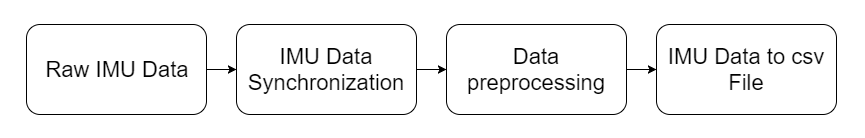
\includegraphics[width=\linewidth]{figures/imuflow.png}
\caption{Diagram showing the progression and dependence of the major stages of IMU data processing in this project}
\label{fig:imuflow}
\end{figure}

From the diagram we can see that our input is a large unprocessed dataset captured by the smartphone with a logging rate of 100Hz. From this critical data must be extracted and synchronized with the rest of the system. The data must also be manipulated to keep units constant and unify various frames of reference. By correctly preprocessing the data, the implementation of the EKF is simplified.

\subsection{Obtaining IMU Data}
Obtaining the raw sensor data was discussed in the 


All these variables have been recorded with respect the smartphone frame of reference as shown below



\subsection{Synchronizing IMU Data}
The AndroSense application can record the the magnitude of sound that the microphone is experiencing. Using this magnitude we can see at what sample the spike from the clap was recorded. This sample will be a common point between the IMU and the cameras and can thus be used to synchronize the different hardware elements.

\subsection{Preprocessing IMU Data}
Before we can apply the IMU data directly to the EKF we need to make some minor modifications to the data. This is critical in removing any bias from the sensors. as discussed in the Sensor calibration section.

in order to extract the linear acceleration from the data we can simply take the measure acceleration and subtract the gravitational acceleration vector

\subsection{Exporting IMU Data}
The IMU data was finally exported as a csv final and imported into MATLAB as different vectors. This allows for faster processing and better data processing in matlab.





\section{Processing the Video Data}
To once again simplify the design and implementation of the EKF it is important to pre-process the video data to a less data heavy format suc as MP4. The following digram shows the process of converting a large video file to a more lightweight csv file without losing any critical information.

\begin{figure}[!ht]
\captionsetup{width=0.8\linewidth, font=small}  
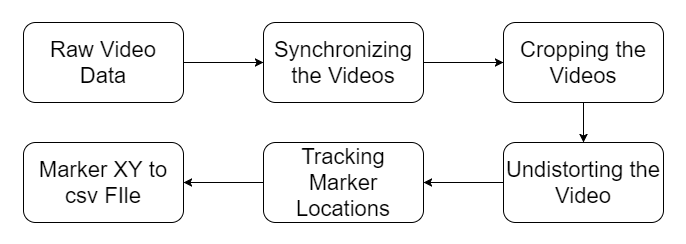
\includegraphics[width=\linewidth]{figures/videoProcess.png}
\caption{Diagram showing the progression and dependence of the major stages of video processing in the project}
\label{fig:videoProcess}
\end{figure}

All raw video data streams must be synchronized and the important sections of the streams extracted. Correcting the various distortions introduced by the lens properties of the GoPro  and decompressing the video files are necessary before image processing is attempted. Finally each marker position in every frame of all the individual cameras must be quantified. These pixel coordinates will serve as inputs to the EKF. 

\subsection{Obtaining Video Data}
The cameras were configured as outlined in the previous chapter. go pro remote start them all recording video at the same time



\subsection{Synchronizing Video Sources}
I typical problem faced when working with different sources of data is that of synchronization. Since this project used 4 different cameras, synchronizing the video sources are critical to generate accurate stereo vision data.

The problem of synchronization was overcome by using a audio cue to align the video data post capturing. With all systems recording, a simple hand clap can serve as a spiking audio input easily identified in the audio track of the video streams. The frame associated with this audio spike can be identified using SVP (Sony Vegas Pro) video editing software as shown in the figure below. 

\begin{figure}[!ht]
\captionsetup{width=0.8\linewidth, font=small} 
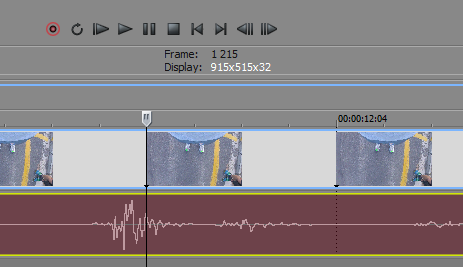
\includegraphics[width=0.5\linewidth]{figures/svpframe.png}
\caption{Figure showing the user interface of SVP video editing software}
\label{fig:svpframe}
\end{figure}

The red track in the above figure shows the recorded audio stream while the corresponding frames are displayed in the blue track above that. The cursor is aligned with the audio spike caused by the clap with the corresponding frame number displayed below the playback controls.

This method was repeated for every video stream such that a common starting point was generated. 

\subsection{Cutting Critical Video Data}
With the video data synchronized the next step was to generate a subset of video demonstrating a transient period and steady state period of running. From accelerometer readings we can easily determine the gait cycle period of our subject; that is the amount of time take between the same foot impacting the ground. These impacts are visible as spikes as seen in the accelerometer data.  

\subsection{Undistorting the Video Data}
To generate accurate distances using stereo vision the video frames need to be undistorted.

Distortion of the frames is a result of the 

To gain further understanding of undistorting video files \cite{Hartley2004} served as a reference. In this work Hartley describes various methods of undistorted images. These distortions are due to various lens effects.

\subsection{Tracking and Exporting Marker Positions in the Frame}

This section discusses the different methods of feature detection subdividing them into two main methodologies: automated and semi-automated. Each of these approaches offer advantages and disadvantages. To understand the approaches considered for this work it is important to visualize the input image data to the system. The following picture shows the various frames from all the cameras.

\begin{figure}[!ht]
\captionsetup{width=0.8\linewidth, font=small} 
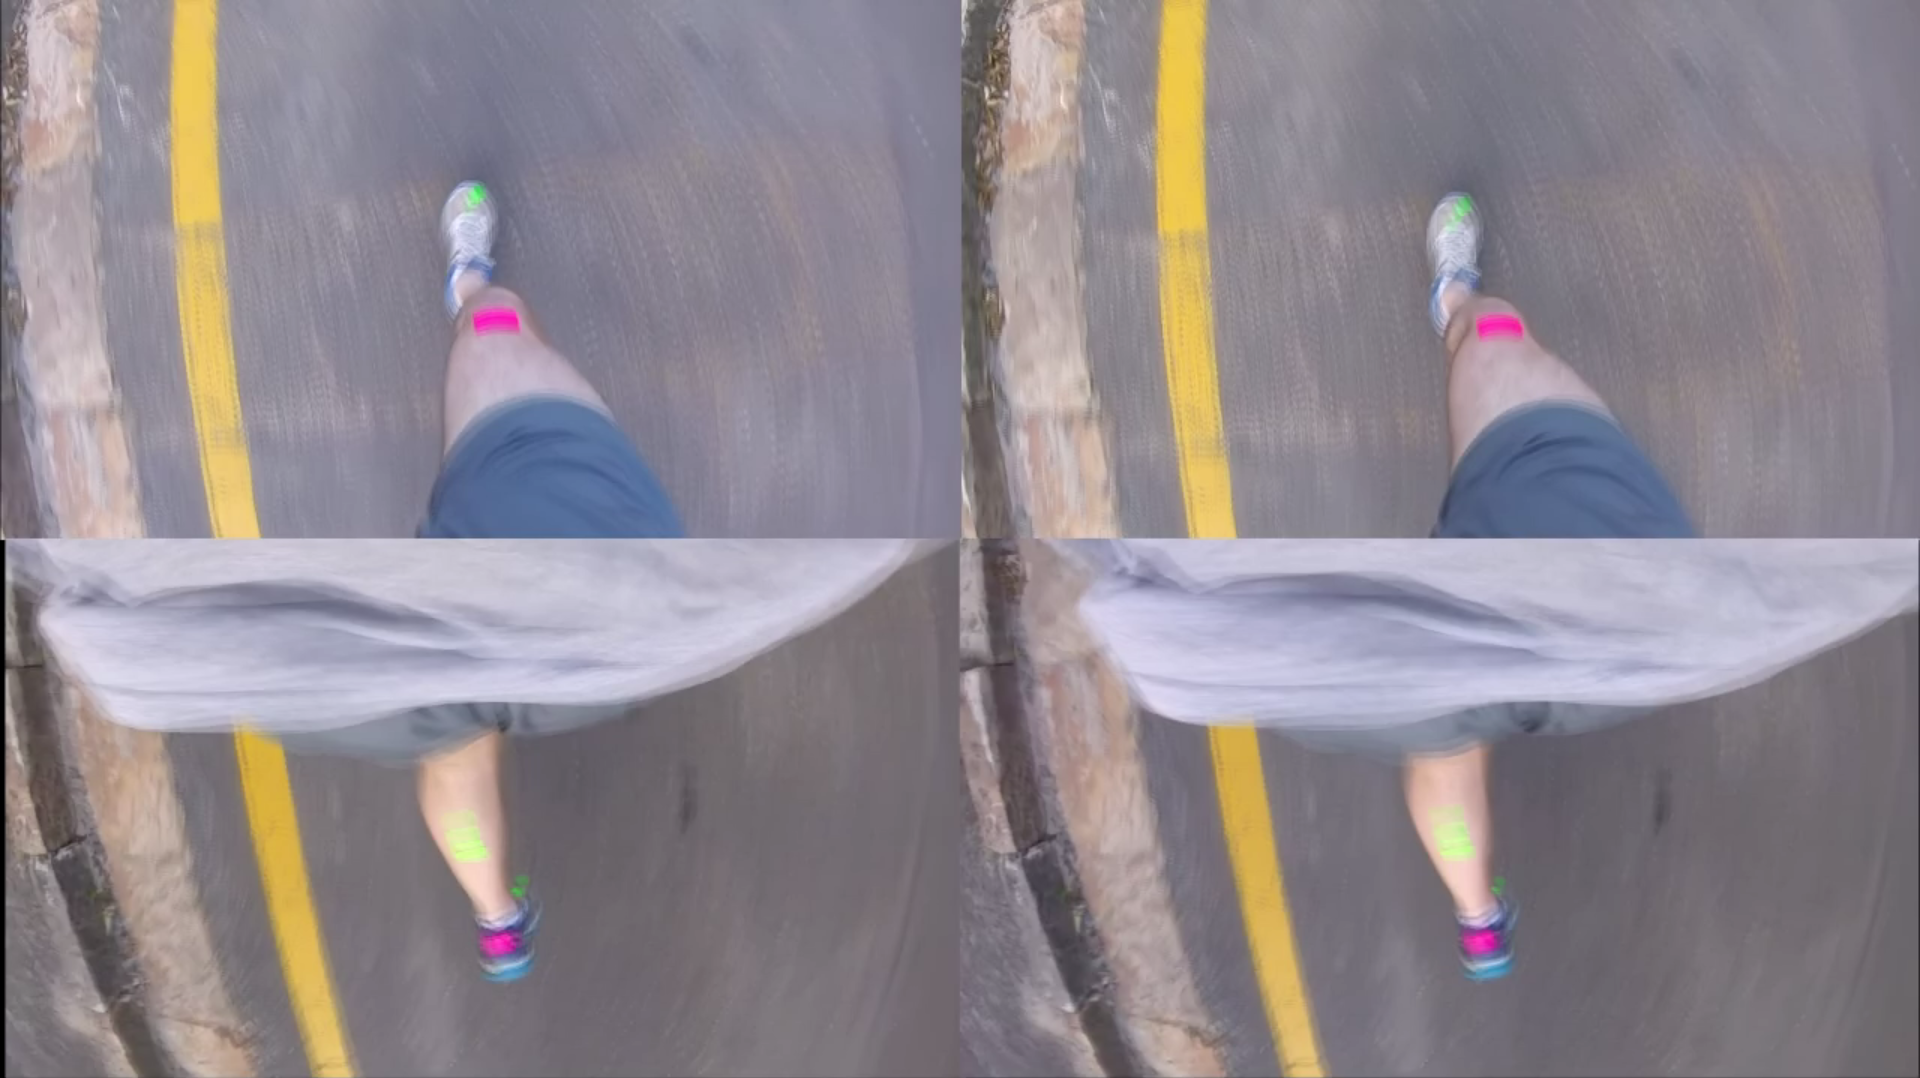
\includegraphics[width=\linewidth]{figures/pat_run_quad.png}
\caption{4 Frames from the different cameras combined}
\label{fig:pat_run_quad}
\end{figure}

The top row of images have been generated by the front mounted cameras and the bottom row by the rear mounted cameras. The left images were produced by the left cameras and the right images by the right cameras. From this image we can get a visual idea of the data our image processing system needs to manipulate.

Feature detection is a methodology in image processing that allows critical points of an image to be detected. This extracts an XY coordinate of the point of interest that can then be used to track the movement and position of object in the image. This methodology can be applied with frames with more than one point of interest as shown in this work. Multiple points of interest in multiple video sources does however increase the complexity of feature detection.

An initial approach of using automated detection was considered and three possible system were considered. Using a trained neural network, using an edge detection algoritm with a panning search algorithm and finally using a colour identifying algorithm paired with a local search algorithm.

In theory a well trained \textbf{neural network} will provide the most robust and accurate system to identify features in varying lighting condition. It would also be the most accurate methodology for a system without the markers. This is due to the \textit{understanding} developed by the neural network after sufficient training data is processed.

This however presents a key difficulty in setting up and training a neural network. The most important element of a neural network is the training data used to teach the. This training data needs to have annotated images with metadata fields to

A neural network therefore cannot generate training data and a method of generating training data needs to be considered in any case.

The second approach taken was that of \textbf{edge detection}. This method 

The final approach considered and used was to \textbf{semi automatically} label critical point in the image using a toolbox created by Hedrick et al. \cite{hedrick2008software}. This software allows for a semi automatic tracking of points of interest in the video frames. While this method is labour intensive it is arguably more accurate than the previously investigated methodologies. The following figure shows the functionality of the toolbox within MATLAB.

\begin{figure}[!ht] 
\captionsetup{width=1\linewidth, font=small}  
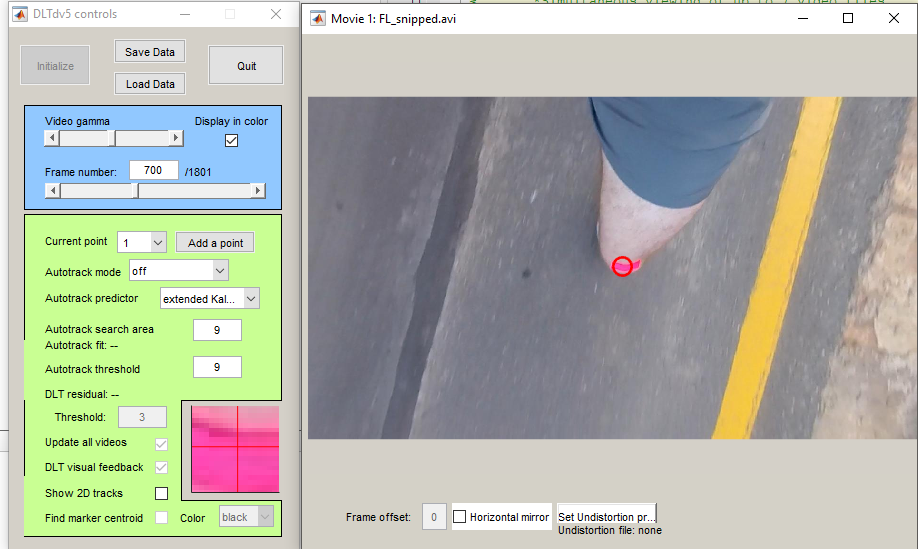
\includegraphics[width=1\linewidth]{figures/toolbox.png}
\caption{Using the dltdv toolbox in MATLAB to export marker coordinates}
\label{fig:toolbox}
\end{figure}

By using this toolbox we can generate a dataset of $ (x,y) $ pixel coordinates by identifying the different markers on each frame and assigning their corresponding points to them. The following tables shows the markers and their corresponding point.

\begin{table}[!ht]
\centering
\caption{Table showing the relation between points and markers}
\label{my-label}
\begin{tabular}{ll}
Front Cameras &            \\
Point 1       & Right Knee \\
Point 2       & Left Knee  \\
Point 3       & Right Foot \\
Point 4       & Left Foot  \\
Rear Cameras  &            \\
Point 1       & Right Calf \\
Point 2       & Left Calf  \\
Point 3       & Right Heel \\
Point 4       & Left Heel 
\end{tabular}
\end{table} 


\section{On units}
In order to assure consistency between the different sources of data considering a general set of units is of critical importance. It was decided to implement the system using SI units such that all lengths was given in meters and all angles in radians.

gyroscope was logged as radians per second,

accelerometer was logged as meters per second .

imgae data was recorded as m

\section{On Frames of Reference}
we need to developed some commonalities among the various sensors and their individual frames of reference. The body frame

\begin{figure}[!ht] 
\captionsetup{width=0.5\linewidth, font=small}  
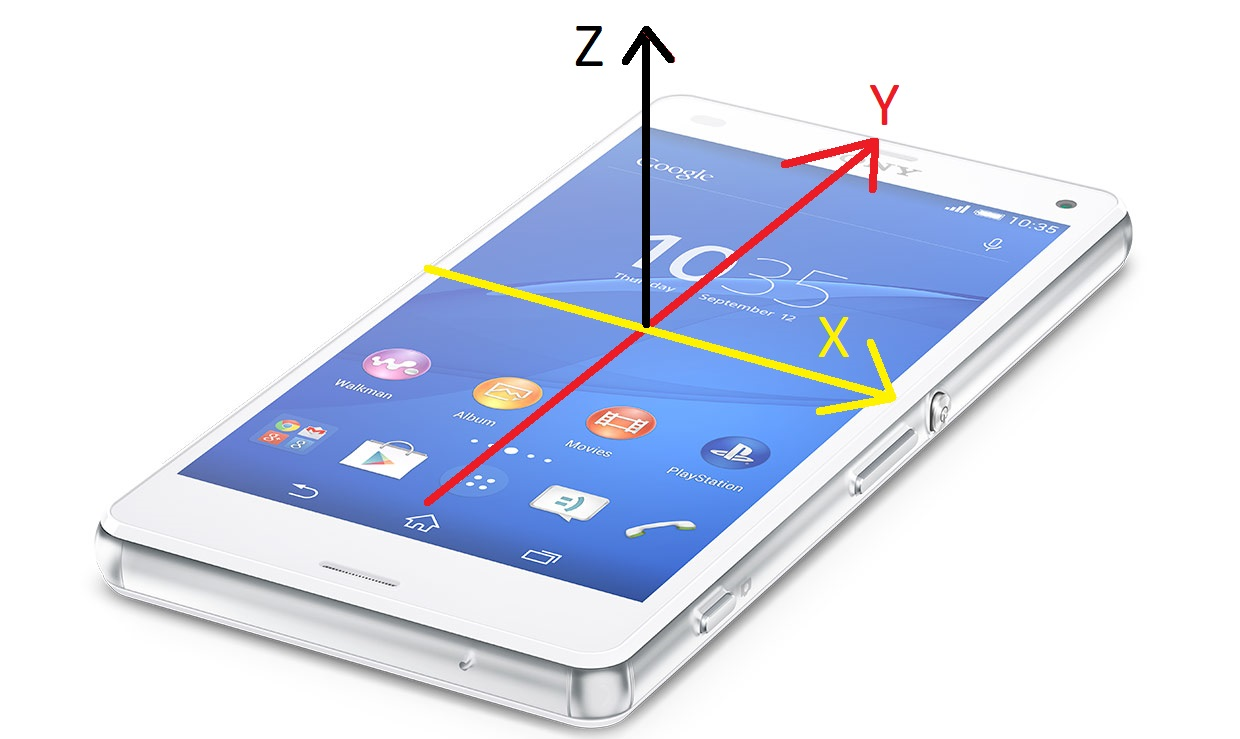
\includegraphics[width=0.5\linewidth]{figures/phone.jpg}
\caption{Figure demonstrating the frame of reference of the smartphone}
\label{fig:phone}
\end{figure}









